\section{Sensorenhet}
Sensorenhetenutgörs av en AVR microcontroller samt de analoga sensorer som är kopplad till denna. Sensorenheten har till uppgift att samla in information från omgivningen via sensorer samt tolka den insamlade datan. I autonomt läge kommer sensorenheten ta direkta styrbeslut baserade på denna data. 

\subsection{Hårdvara}
Sensorenheten består av en AVR ATmega16 som kopplats till 3 avståndssensorer, de sensorer som hittar linjer på marken samt en display. ATmega16 har en intern AD-omvandlare på Port A som kommer användas.

\subsubsection{Linjeföljarsensor}
Linjeföljarsensorn utgörs av en reflexsensormodul kopplad till en mux och en demux av typen 4067. Reflexsensormodulen består av 11 lysdioder och 11 ljuskänsliga transistorer.  Muxarna styrs av AVRen och får lysdioderna och transistorerna att arbeta i par. Den ena muxen är kopplad till logiskt ett på sin ingång för att tända en lysdiod i taget, demuxen kopplar motsvarande transistor till A/D omvandlaren. Efter att en omvandling är klar kopplas muxarna om till nästa par och en ny omvandling kan starta.

\subsubsection{Avståndssensorer}
Sensorenheten har 3 optiskaavståndsmätare av typen GP2Y0A02YK (20-150 cm). En placerad på vardera sida av roboten och en riktad frammåt. Dessa ger en analog utsignal som kopplas till AVR:ens AD omvandlare och tar upp en pinne var.

\subsubsection{Display}
En alfanumerisk LCD-display av typen HD44780U används för att visa avstånd till väggarna när roboten är i labyrintläge. Displayen körs i sitt 4 databits läge och kopplas till Port D på AVR:en, 7 pinnar.


\subsection{Mjukvara}
Robotens styrbeslut fattas i autonomt läge av sensorenheten. 

\subsubsection{AD}
De 8 mest signifikanta bitarna från ATmegas inbygda AD omvandlare kommer att användas efter varje omvandling. Alla sensorer kommer i turordning omvandlas. När en omvandling är klar läses data ur ADC Data Registers och sparas i ett annat register varefter nästa omvandling startas. En räknare kontrollerar vilken av de 3 avståndssensorerna och de 11 linjesensorerna som AD-omvandlas igenom att ställa in interna och externa muxar.

\subsubsection{Linjesensor}
När AD-omvandlaren har gått igenom alla linjessensorer ett varv kommer värdena från linjesensorerna trunkeras. Trunkering ska ske så att tejp kommer motsvara en etta och ingen tejp en nolla. Med detta går det att räkna fram hur långt till höger eller vänster roboten befinner sig om linjen. I autonomt läge skickas avståndet till Styrenheten som reglerdata och till PCn för visning.

Om alla sensorer visar tejp i autonomt linjeläge kommer kommandot "kör rakt fram" skickas till Styrenheten och PC.
Om roboten befinner sig i autonomt labyrintläge och läser av en bred svart tejp kommer en intern klocka startas för att mäta hur lång tejpen är. Värdet matchas sedan mot en tabell med data och motsvarande styrkommando sparas.

\subsubsection{Avståndsberäkning}
Värdena från AD-omvandlingen av avståndssensorernas data omvandlas enligt en tabell till avstånd. Dessa visas direkt på på den externa displayen. Avstånden kan sedan användas för att ta fram vart roboten befinner sig relativt mitten av banan. Detta värde skickas till styrenheten.

Om avståndet till en vägg är större än 80 cm så undersöker sensorenheten om det finns ett sparat styrkomando, om det finns skickas det sparade styrkommandot, annars ett svängkommando.

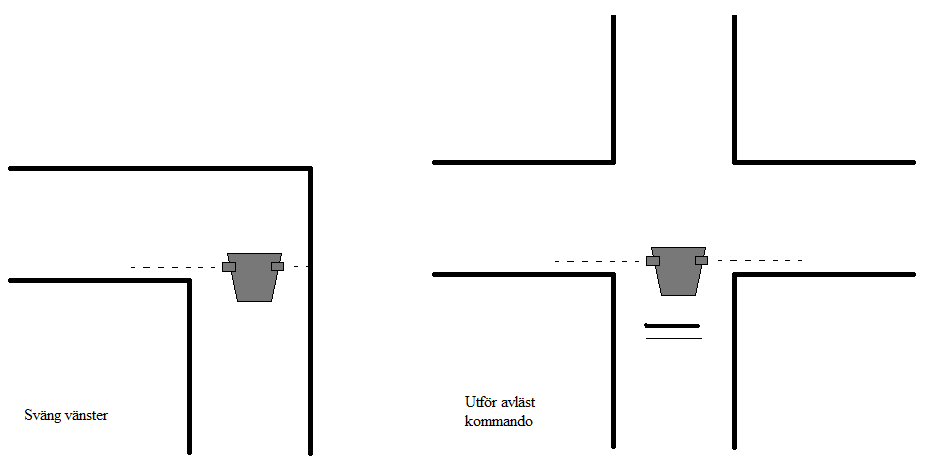
\includegraphics[angle=0,scale=0.5]{bilder/labkors.png}

\subsubsection{Kommunikation}
Port B på AVRen kommer användas för SPI bussen. Sensorenheten kommer skicka en interuptsignal till Kommunikationsenheten för att starta en överföring.

